\chapter{bubbleRob 機器人建立}
\section{將Coppeliasim版本更改為可執行python程式}
\begin{figure}[hbt!]
\begin{center}
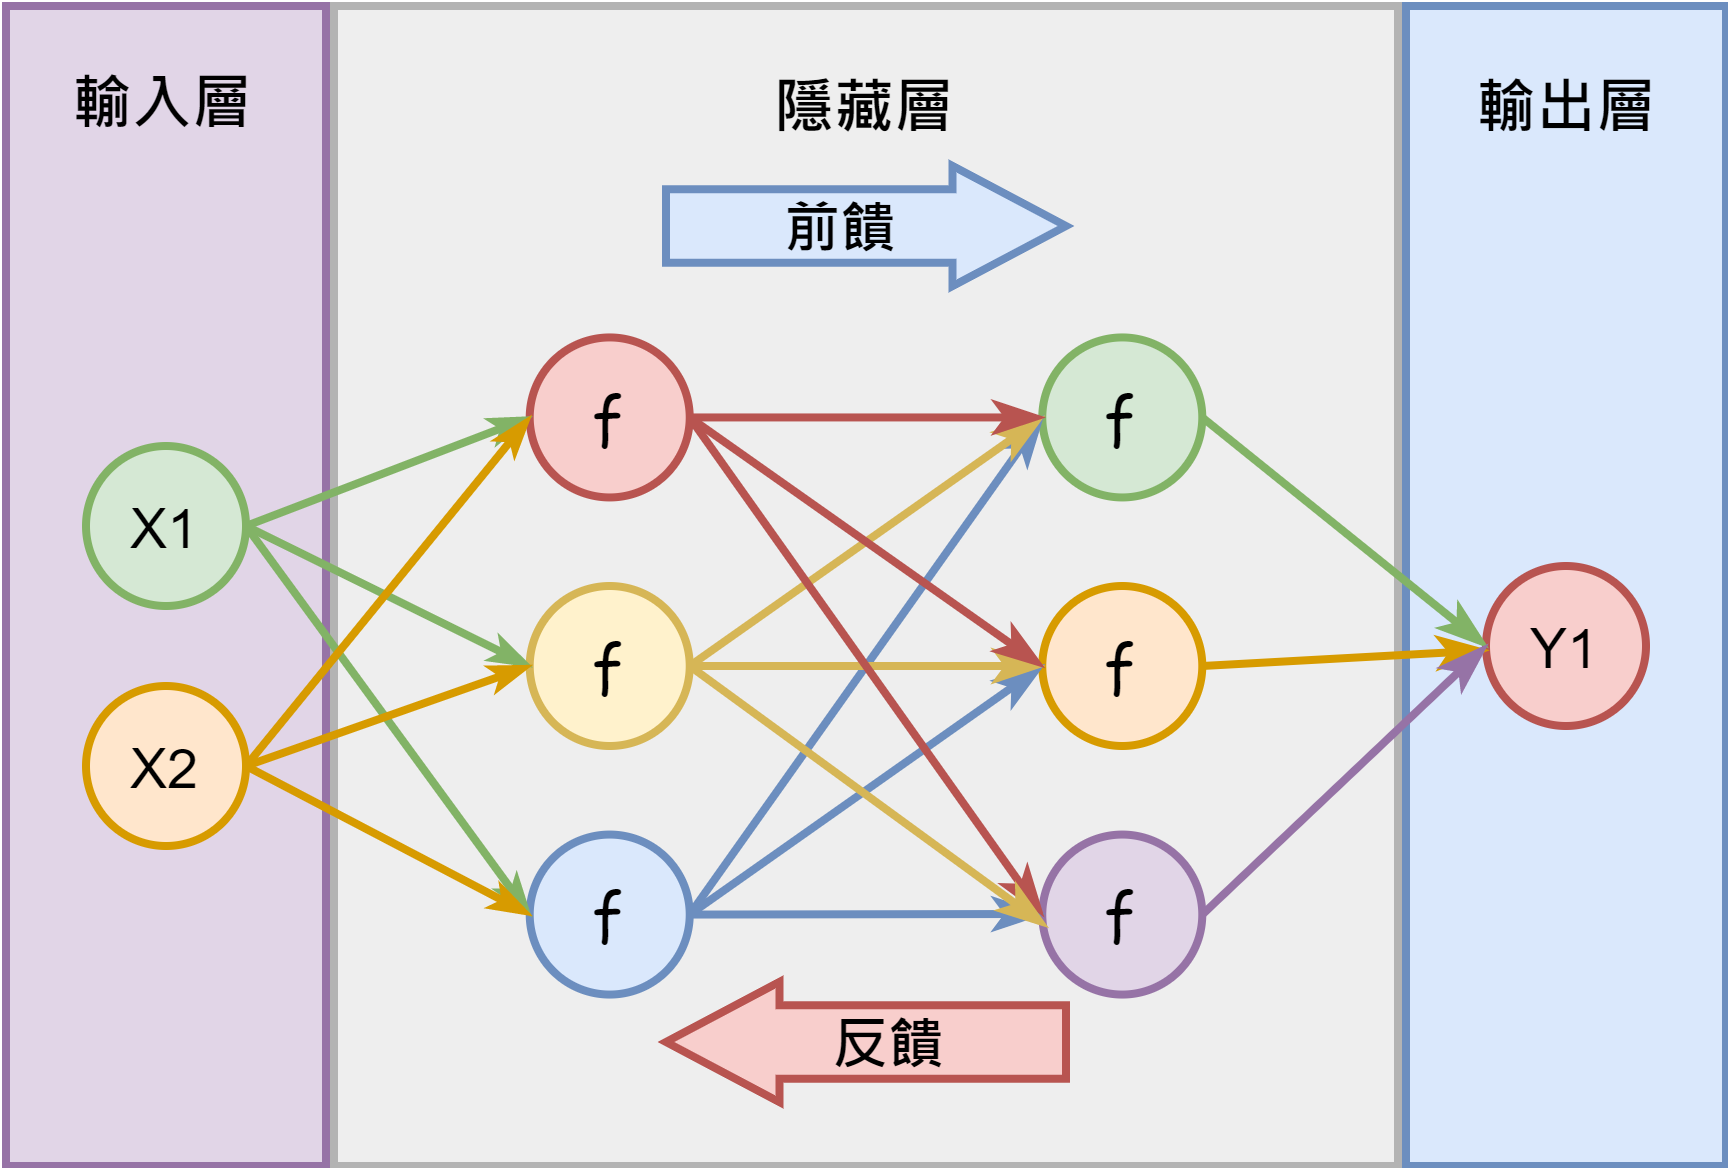
\includegraphics[width=16cm]{類神經網路架構}
\caption{\Large 設定 }\label{ 設定 }
\end{center}
\end{figure} 
 CoppeliaSim 自 4.3 版之後除了 Lua scripting, 增加了 Python scripting 功能. 但是必須在 usrset.txt 中設定 defaultPython 指向 Python.exe, pip install cbor zmq, 並且設定 executeUnsafe = true. 完成後開啟 CoppeliaSim 4.3.0 rev12, 並利用 scenes/simplePythonExample.ttt 進行測試  如(圖.\ref{ 設定 }) 。\\


\newpage
\begin{figure}
\begin{center}
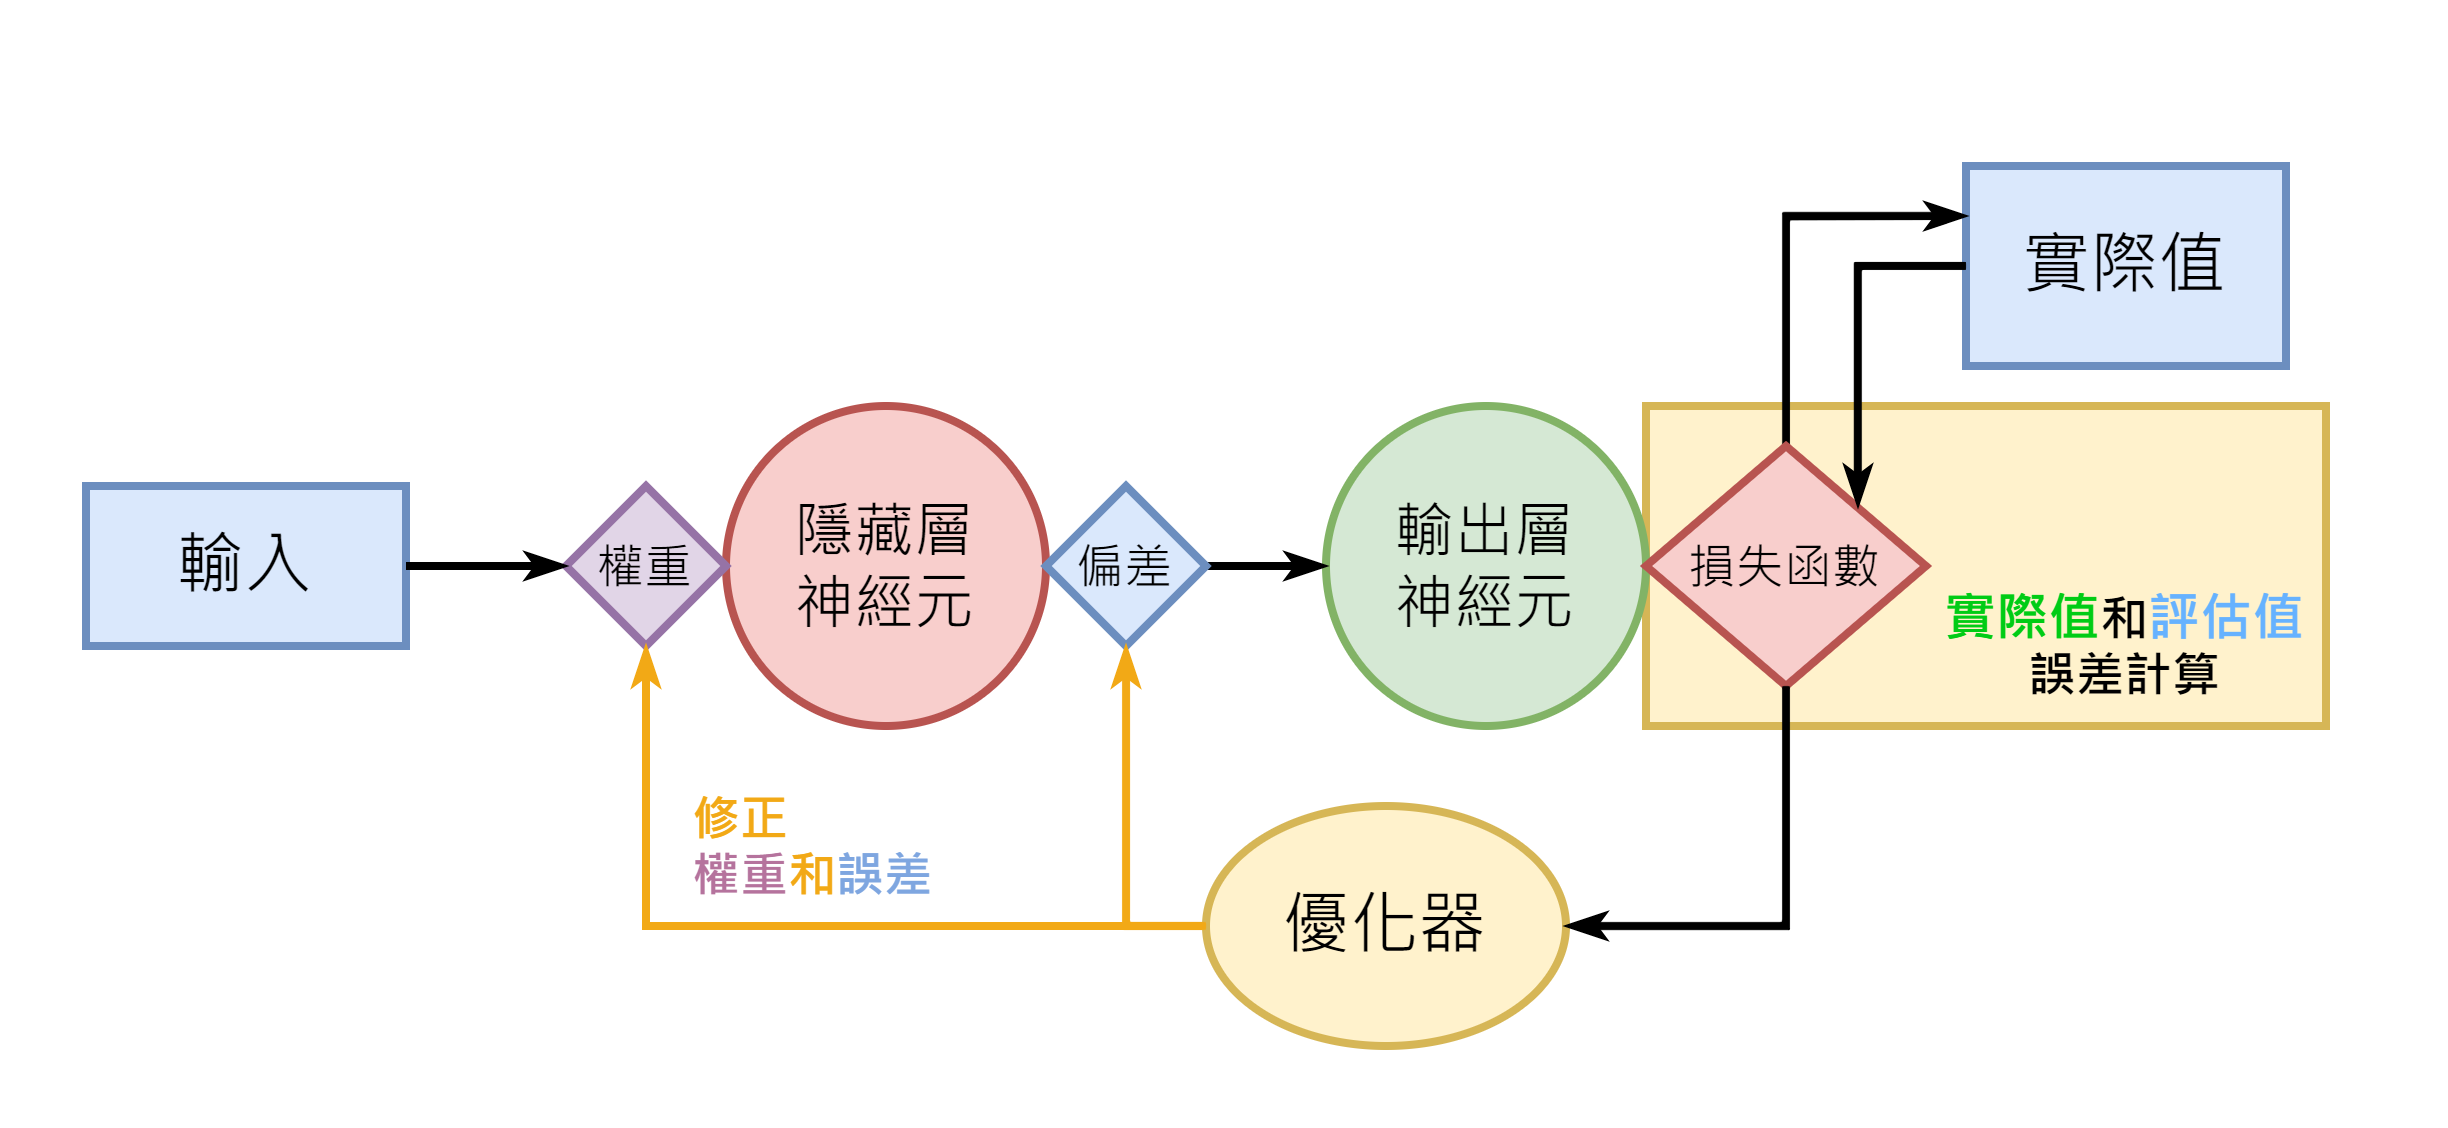
\includegraphics[width=16cm]{類神經網路關係}
\caption{\Large 本體建立}
\label{本體建立}
\end{center}
\end{figure}
\section{本體建立}
本體如(圖.\ref{本體建立}) 及感測器是進行專案的重要基礎,各項參數要設定得宜才能得到正確的結果。\\
以下介紹幾種較為常見的參數設定及其特性:
\begin{itemize}
%=----------Body is respondable----------=%
\item Body is respondable (圖.\ref{Body is respondable 、Body is dynamic}):\\
respond是回答,回應的意思。可響應形狀將導致與其他可響應形狀的碰撞反應。即respondable屬性用於控制物體的碰撞回應,nonrespondable物體在與其它物體發生碰撞時,物理引擎不會進行計算,會出現穿透的現象。

%=----------Body is dynamic----------=%
\item Body is dynamic (圖.\ref{Body is respondable 、Body is dynamic} )是具有動態屬性的物體會在重力影響下墜落或在其它外力、力矩作用下發生運動狀態的改變。而靜態物體則會在場景中靜止不動,如地面,或跟隨其父節點運動(或跟隨其父節點在場景層次結構中的移動)。\\
\begin{figure}[hbt!]
\begin{center}
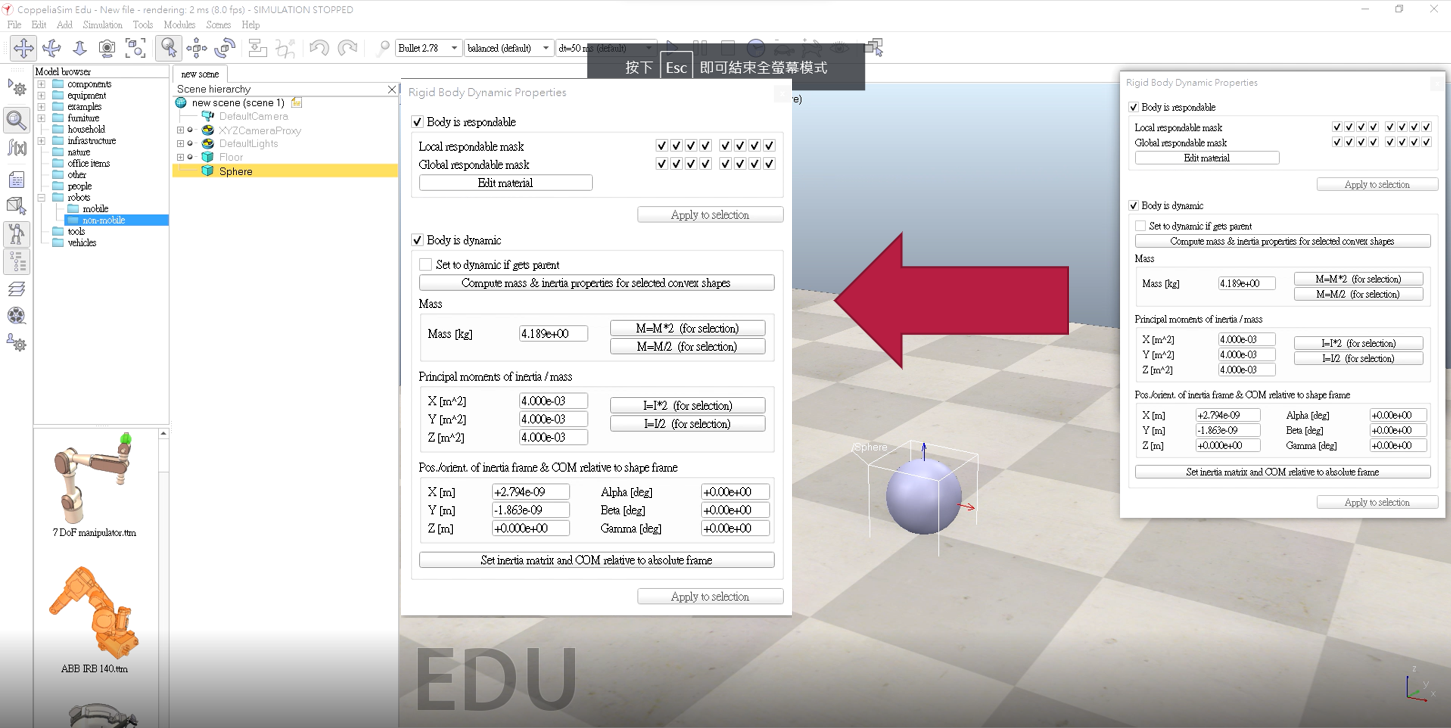
\includegraphics[width=16cm]{SigmoidFunction}
\caption{\Large Body is respondable 、Body is dynamic}\label{Body is respondable 、Body is dynamic}
\end{center}
\end{figure}
\\
\\
%=----------Collidable----------=%
\item Collidable(圖.\ref{Collidable、Measurable、Detectable}):\\
碰撞檢測,可以檢測兩個碰撞體實體(Collidable objects are objects that can be tested for collision against other collidable objects)之間的碰撞,類似於SolidWorks等三維設計軟體中的干涉檢查。 碰撞檢測只會檢測碰撞狀態,而不會直接對碰撞做出反應(The collision detection module will only detect collisions; it does however not directly react to them)。 碰撞檢測模組中可以註冊碰撞物件,即collidable entity-pairs (collider entity and collidee entity). 在模擬過程中,註冊的碰撞對象之間的碰撞狀態可以由不同的顏色可視化顯示,也可以通過Graph來進行記錄。
%=----------Measurable----------=%
\item Measurable(圖.\ref{Collidable、Measurable、Detectable}):\\
通常指可以測量的物理量或仿真參數,例如機器人的位置、速度、加速度、力和角度等。這些可測量的量可以用來監測機器人的行為,評估控制算法的性能,或者用於自動化調整機器人的運動。\\
%=----------Detectable----------=%
\item Detectable(圖.\ref{Collidable、Measurable、Detectable}):\\
指可以被檢測到的物理量或仿真參數,這些可檢測的量可以用來檢測機器人與周圍環境的交互,例如檢測是否有障礙物、檢測是否接近目標等。\\
\begin{figure}[hbt!]
\begin{center}
\includegraphics[width=16cm]{三要素}
\caption{\Large Collidable、Measurable、Detectable}\label{Collidable、Measurable、Detectable}
\end{center}
\end{figure}
\\
\end{itemize}
\newpage
